\subsection{Trustable}
La confianza entre la plataforma que queramos utilizar y el usuario tiene que ser firme.
Por ello tendremos que garantizar la proteccion de su intimidad y darle la certeza que si 
utilizamos sus datos es solo exclusivamente para un fin en especifico y le dejaremos claro,
cual es ese fin, es decir, transparencia. 
Deberemos por ello minimizar el riesgo de la divulgacion de sus datos, es decir, guardar
por su seguridad, integridad y confidencialidad. 
Para ello deberemos seguir tanto las normas legales como una etica de buenas practicas.
No obligar a un identificado si se puede mostrar informacion.
Siempre pedir permiso para la captura de datos y dejar claro la finalidad de estos.


\subsubsection{How to solve it} 
Utilizacion de plataformas seguras, como puede ser SSL si desarrollamos una aplicacion web.
Si utilizamos API de terceros, asegurarnos tanto de su reputacion como el nivel de seguridad que ofrece.
Implementar un sistema que no permita relacionar los datos con un usuario.
Dar al usuario la posibilidad de eliminar sus datos si asi lo desea.


\subsubsection{How we solve it. Aire Guru} 
En nuestro caso la seguridad es primordiarl ya que para nuestra funcion estrella, el historial personal
de la exposicion a la contaminancion, no es imprescindible recolectar la posicion del usuario.
Para alcanzar un nivel de seguridad competente se ha utilizado SSL, que garantiza la encriptacion de 
la informacion enviada atravez de la red.
Para la identificacion del usuario se ha utilizado un API segura y probada, utilizamos la identificacion
que nos proporciona Firebase. Esta API nos proporciona un identificador, el cual puede ser encriptado o no.
Nosotros hemos utilizado por supuesto el encriptado. Cuando los datos alcanzan nuestra base de datos, 
comprobarmos el usuario y si es correcto volvermos a encriptar el usuario con nuestra propia clave para
asi evitar que se pueda relacionar la base de datos de firebase con nuestra base de datos.

Respecto a la posicion del usuario, nunca almacenamos su posicion exacta, solo el poligono en el que se encuentra
y tambien implementamos un minimo de tiempo. Esto nos permite tener la precision necesaria para mostrarle su 
exposicion a los contaminantes pero no un seguimiento del usuario.

Siguiendo el codigo de buenas practicas, nunca se empieza a recolectar la posicion del usuario sin su permiso,
para ello necesitamos una accion explicita. En nuestro caso, el propio usuario tendra que seleccionar "Mi 
ubicacion" y acceptar que leamos su posicion. Por supuesto el usuario puede siempre revocar este permiso y 
eliminar sus datos en cualquier momento desde la seccion de configuracion.\\

\newpage
\begin{figure}[ht]
    \centering
   \subfigure[Location Access]
    {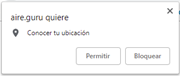
\includegraphics[width=5.5cm  ]{locationAccess}}
    \hfill
    \subfigure [Settings]
       { 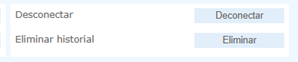
\includegraphics[width=5.5cm]{settings}}
   
  \caption{Filters}
    \end{figure}

La recoleccion de datos de posicion no es exhaustiva, pero garantiza la precision.\\

Como queremos una herrmienta transparente, le explicamos al usuario para que necesitamos sus datos antes
de identificarse, y por supuesto, la identificacion es opcional.\\


\begin{figure}[ht]
    \centering
    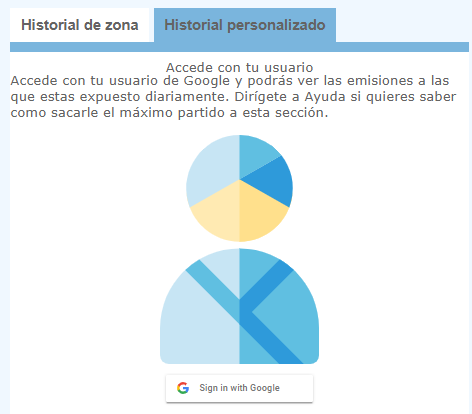
\includegraphics[width=8cm]{loginInfo}
    \caption{Info before login}
\end{figure}


\elsparagraph{Evaluation}  
\begin{itemize}
    \done Codigo de buenas practicas
    \done No es posible relacionar la identificacion del usuario de firebase con nuestra base de datos
    \crossed Algunos usuarios nos indicaron que preferirian crear una cuenta con un nombre de usuario y contrasena
    y no utilizar su cuenta de correo por miedo al "robo de informacion"
    
\end{itemize}
\newpage